\section{The user stories we were assigned}
For sprint 2 we were assigned two user stories to implement on top of our responsibilities as PO.
In the following section we give a short introduction to Flutter, the work flow followed by the GIRAF project and how we implemented the stories.

\subsection{Introduction to Flutter}
Flutter is built on the concept of widgets. Widgets describe what their view should look like given their current configuration and state\cite{Flutterwidget}. 
They are classes to build UIs, used for both layout and UI elements.
Composing simple widgets lets you build complex widgets to create a layout\cite{Flutterlayout}.
Widgets typically extend either the \texttt{StatelessWidget} or \texttt{StatefulWidget} classes from the Flutter library.
\\\\
The difference is that \texttt{StatefulWidget} has the concept of a state within the widget, meaning it can change during the lifetime of the widget.
\texttt{StatefulWidgets} are used when part of the UI can change dynamically.
\texttt{StatelessWidgets} conversely do not have states, meaning they are useful when part of the UI does not depend on anything other than the basic information of the widget. 
The basic widgets used to create a layout are\cite{FlutterBasicWidgets}:
 \begin{itemize}
    \item Container
    \item Row
    \item Column  
    \item Scaffold
    \item Text
    \item Image
    \item RaisedButton 
 \end{itemize} 
Most of these widgets are self explanatory. 
Rows let you layout a list of child widgets in the horizontal direction, columns let you do that in the vertical direction.
Container lets you customize its child widgets with, for example, margins or borders.
Scaffold helps structure the application, for example, by determining where to place the top bar.

\subsection{The architecture of GIRAF}
The architecture of GIRAF us built on separate blocks to create functionality. 
The overall architecture is illustrated in \autoref{fig:architecture-giraf}.
\begin{figure}[h]
  \centering
  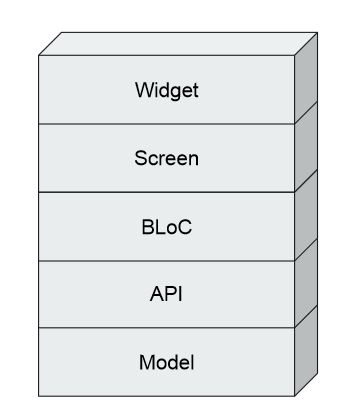
\includegraphics[width=0.3\textwidth]{girafarchitecture.JPG}
  \caption{The architecture of GIRAF}
  \label{fig:architecture-giraf}
\end{figure}
As show, the bottom layer is the model. 



\subsection{Our user stories and how we implemented them}
For sprint 2 we were assigned the following user stories:

\begin{itemize}
    \item "As a citizen I would like to be able to view my week plan so that I know what is going to happen"
    \item "As a guardian I would like to be able to view a given citizen's week plan so that I can get an overview of what is happening this week for them"
\end{itemize}
These user stories define essential functionality for the week planner - actually viewing the plan for both guardians and citizens.
This means we needed to implement the design for the basic view of the week planner, as defined by our prototypes.
The following prototypes show the plan for the design:




